\chapter{Sherbrooke's way of life}\label{ch:ch4label}

Orientons-nous sur la vie à Sherbrooke. Parce que les études c'est bien, mais si le cadre n’est pas cool, autant restez chez soit!

\section{Le débarquement}\label{sec:sec4.1}
Si vous avez bien pris vos précautions sur les documents à fournir lors de votre arrivée, et que vous vous êtes muni d'accueil plus, alors tout ira très rapidement. Pour vous dire, j'ai mis 15 minutes à sortir de l'aéroport, recherche de valises comprise! À l'arrivée, vous serez dirigé vers les bureaux de la douane ou une personne vous remettra votre permis d'étude.


\begin{example}{Un document manquant et c'est retour au bercail}
  Pour la petite histoire, j’ai vu des Français se faire refuser l’accès, car il n’avait pas leur permis d’étude. \textbf{Le CAQ seul NE SUFFIT pas.} Ne tentez pas votre chance en vous disant que ça passe, vous ferez le tour du poteau comme tout le monde.
\end{example}


\section{Les paysages et les Québécois}\label{sec:sec4.2}
Si vous aimez la nature et les beaux paysages, vous allez adorer la vie au Canada, je ne vous en mets pas des images, car vous les trouverez sur Google Images ou vous ferez une visite guidée sur Google Maps, mais c’est vraiment beau.
Pour ce qui est des gens, ils sont « ben nice »! C’est-à-dire qu’ils sont très calmes, accueillants, souriants et toujours là pour vous aider. Au niveau de l’accent, on s’y fait après quelque temps et ce n’est pas si dépaysant que cela.
Pour ce qui est de la météo, ce qui effraie pas mal de personnes en France, ce n’est pas aussi terrible. Pour l’instant (pour ma part d’août à octobre) je n’ai eu que des journées de folie, l’été est vraiment chaud. Ce qui nous donne pas mal de temps pour faire des activités comme du kayak sur le fleuve Magog (où l’eau est bizarrement chaude elle aussi). Vous trouverez plein de balades en montagne, de la descente en vélo, et du ski en Hiver bref, vous êtes servi côté nature! \\
Pour ce qui est de l’hiver, les avis sont mitigés, je ne peux pas trop me positionner maintenant, mais allez faire un tour sur les sites de météo, on tourne aux alentours des -10C quand on est vraiment dedans, mais les vêtements sont adaptés et les locaux aussi donc ça ne devrait pas être compliqué.


\section{Les appartements}\label{sec:sec4.3}
Pour ce qui est du logement, ne vous en faites pas, vous êtes servie. Vous pouvez trouver un appartement sans aucun problème ici, pour tous les prix. Ne réservez pas un appartement depuis la France par contre, avisez-vous bien de le visiter avant!

\begin{figure}[h!]
\centering
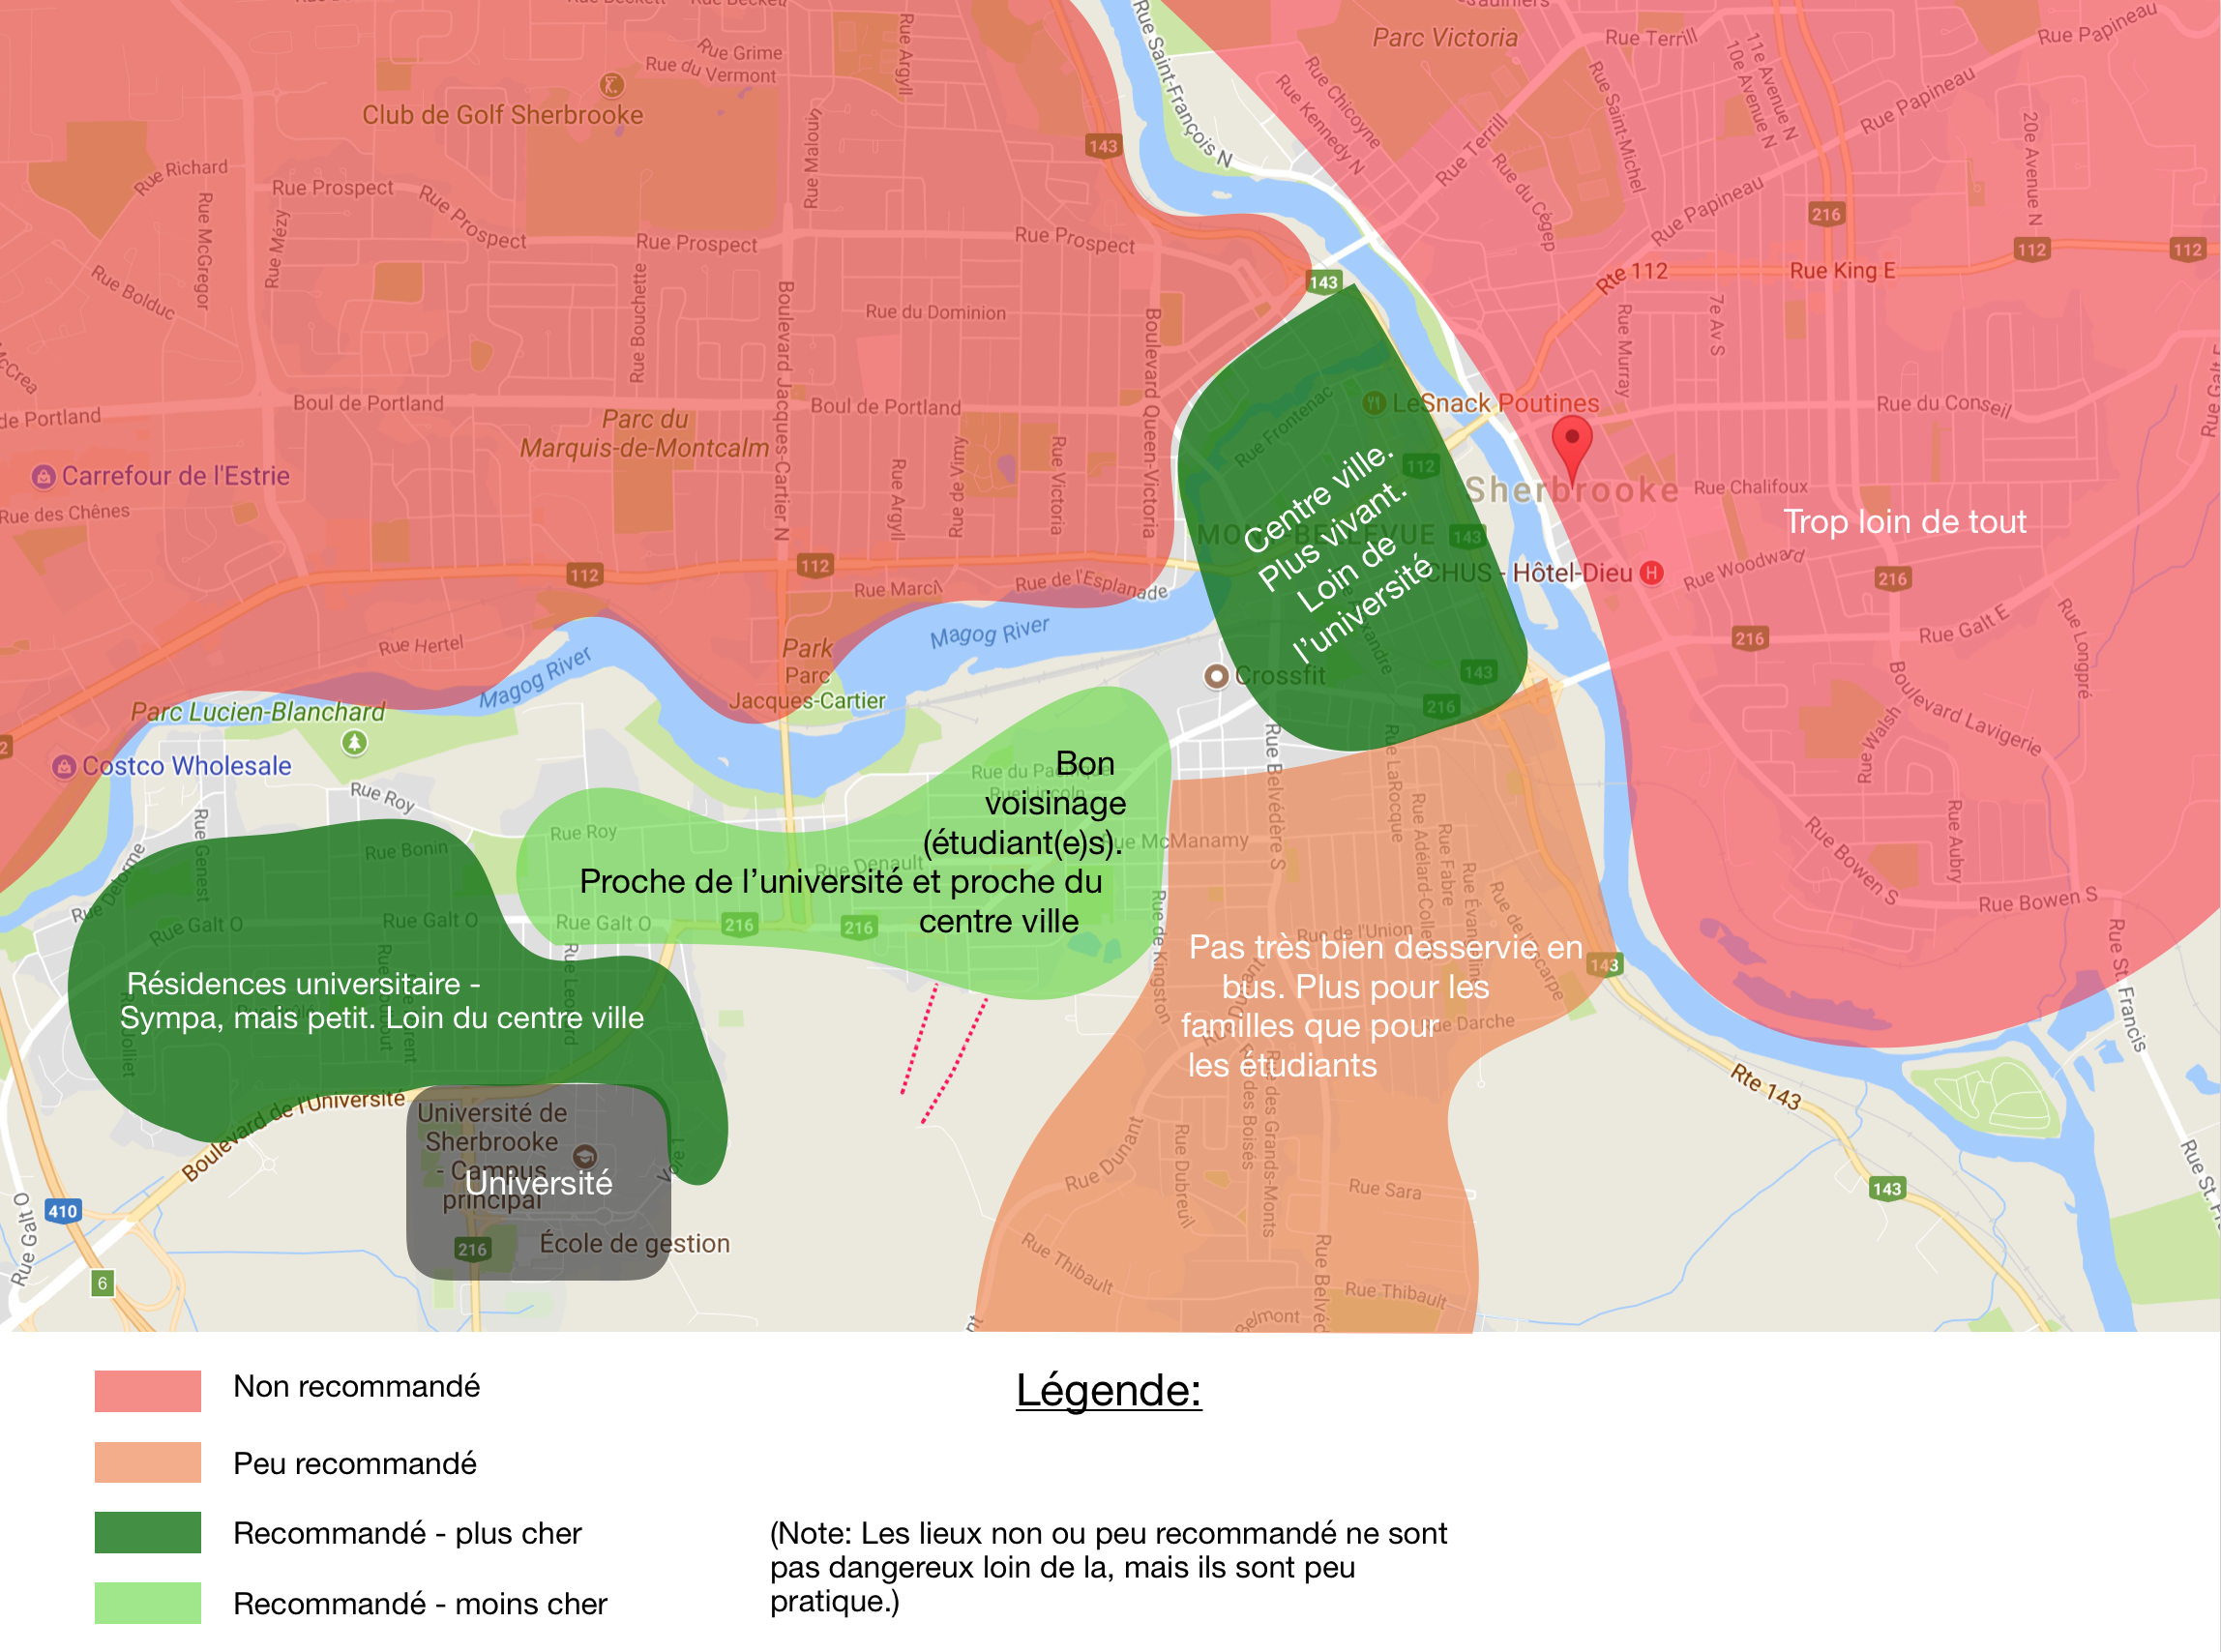
\includegraphics[width = 150mm]{figures/Places_To_Live}
\caption{Selon moi, les zones d'habitations pour vous orienter dans vos recherches}
\end{figure}

\clearpage

\begin{figure}[h!]
\centering
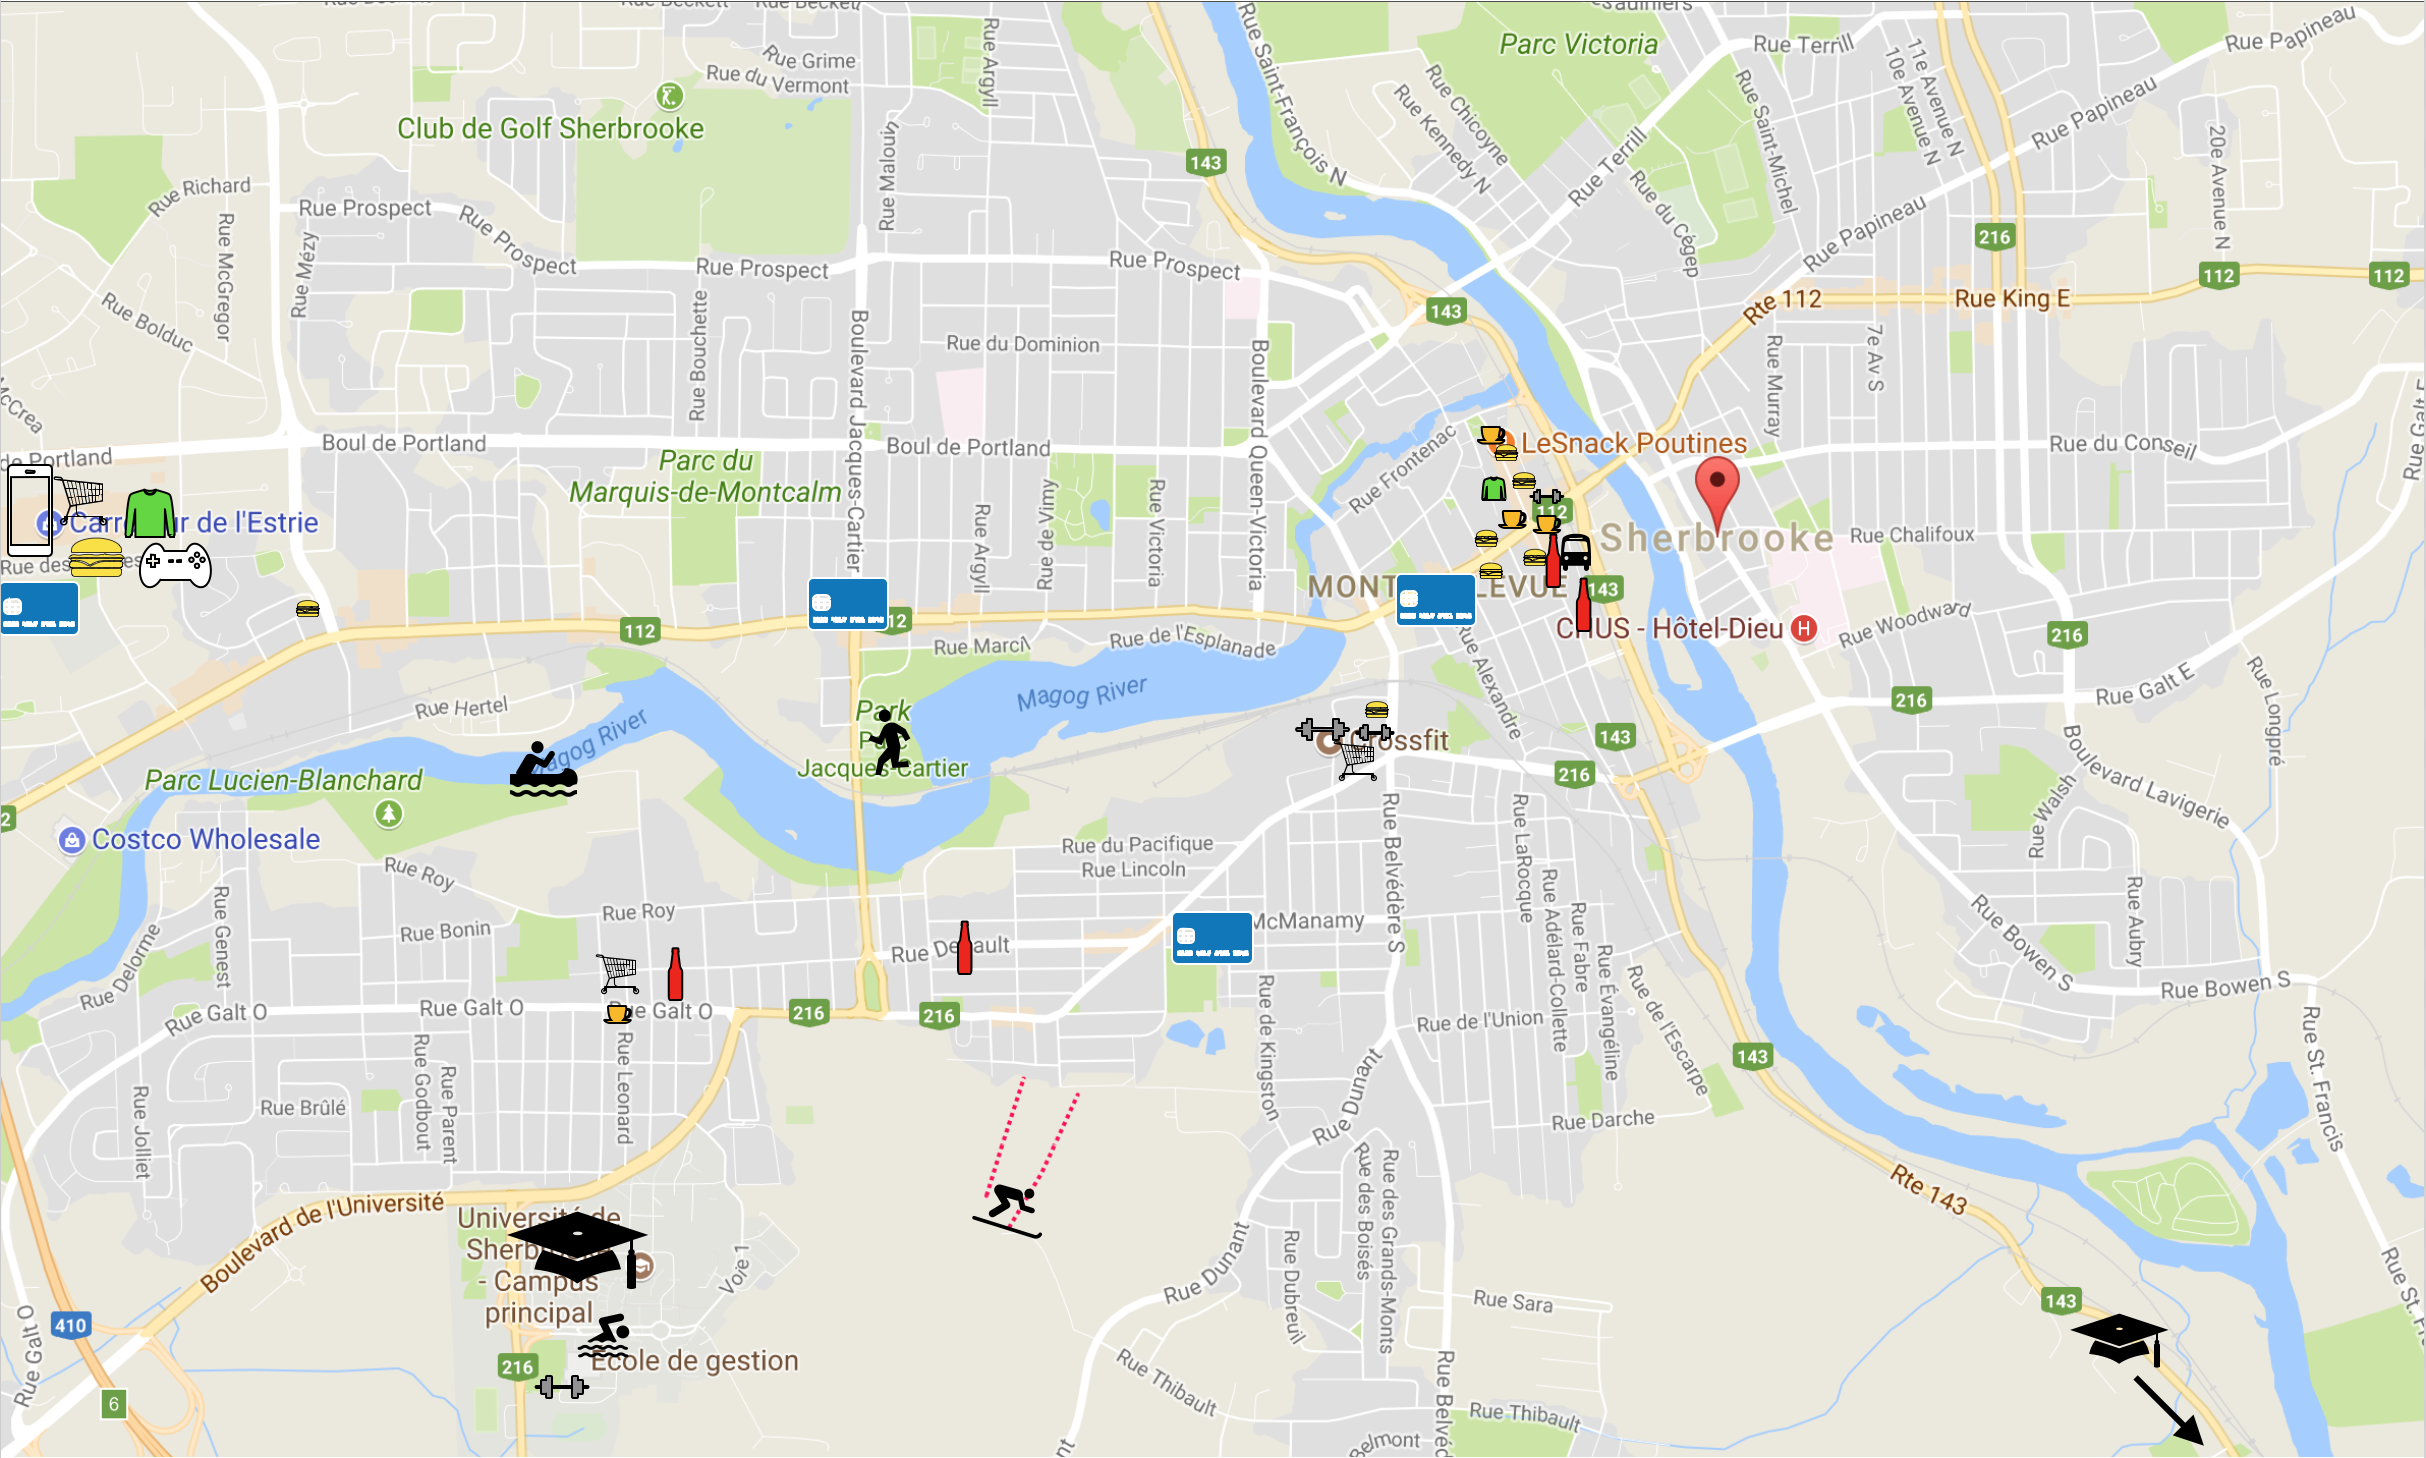
\includegraphics[width = 150mm]{figures/Good_Places}
\caption{Certains endroits sympa à avoir à côté de chez soi}
\end{figure}

Je vous donne le contact suivant qui est notre propriétaire actuellement. Nous y sommes très bien logés et vu qu’il détient deux blocs d’appartement l’un en face de l’autre, qu’il loue principalement aux étudiants, le voisinage y est idéal. Il nous a aussi gentillement meublé l’appartement qui est tout équipé (frigo, machine à laver, sèche linge, lits, bureaux, etc.) ce qui nous a évité pas mal de frais. Si vous êtes trois à partir, cela est parfait pour vous les appartements ont trois chambres. Au canada on dit que c'est un 5/3: 5 pièces, 3 chambres.

Pour information on paie 960\$ CA par mois tout compris. C'est un loyer très raisonnable pour l'appartement!

\bigbreak
Contact: Marc André Ruel \\
Tel : +1 819 919 8998 \\
Email: cmaruel@hotmail.com \\
Adresse des appartements: 1447 Rue Denault - J1H2P9 - Sherbrooke, Quebec
\bigbreak

À savoir une chose importante, assurez-vous d’avoir les frais d’internet et d’électricité compris dans le prix de l’appartement! Sinon votre facture n’en sera que plus grande... Bien plus grande.



\section{Le coût de la vie}\label{sec:sec4.4}

Difficile de bien mesurer le coût de la vie ici comparé à la France. Je dirais qu’avec le taux de change on s’y retrouve plutôt bien, c’est assez similaire \textbf{sauf} sur quelques points comme les forfaits mobiles ou internet.
En effet, le prix des forfaits est incroyablement cher ici, comme il l’était en France avant que Free vienne remettre les choses à plat. C’est-à-dire que chez notre fournisseur Fido, qui sera le seul accessible pour vous en tant qu’étrangers, vous aurez le droit à cela:

\bigbreak
\href{Annexes/Sherbrooke/Forfait_Fido.pdf}{\textbf{Grille de prix Fido}}\textsubscript{  [link]}
\bigbreak

Ca pique hein? Mais il va falloir faire avec. Après la WIFI est accessible et gratuite partout dans les restaurants ou autre.

\bigbreak

Au niveau de la nourriture c’est un peu plus cher, après je suis un gros mangeur... J’en ai pour à peu près 100 \$ CA de courses par semaine i.e. 70\euro{} et j’en avais pour 60\euro{} en France. Si vous êtes végétarien, divisé le prix par deux, car c’est la viande qui coûte cher ici.

\begin{example}{Le tip et les prix HT}
  Ici tous les prix sont HT, ce qui est assez embêtant, car nous ne sommes pas habitués à cela et on se retrouve avec une belle surprise à la caisse. Il faut donc garder cela à l’esprit. \\
  Autre chose, dans tous restaurant ou bar, le pourboire est de mise! Ne l’oubliez surtout pas, car les serveuses/serveurs sont payé une misère si on ne compte pas leurs tips!\\
  Comment calculer un tip? \\
  Rien de plus simple, il vous suffit d’additionner les deux taxes en fin de reçu et arrondissez le pour avoir le tip! Ajouter un peu plus si la/le serveuse/serveur le mérite... \\
  Je voulais vous mettre une photo de ticket de caisse et puis j'ai remarqué que je ne les gardais jamais... Sorry.
\end{example}


\section{Les transports}\label{sec:sec4.5}
Les transports sont assez présents à Sherbrooke, et pour le bus c’est gratuit pour les étudiants de l’université sous présentation de la carte étudiante bien évidemment. Je vous recommande l’application « Vermeille » ou google maps tout simplement pour avoir les horaires de bus, vous pourrez d’ailleurs l’utiliser en France comme test pour savoir si votre appartement est bien placé. Tout est relativement loin tout de même, comptez 30 minutes de bus pour vous rendre du centre-ville au Carrefour de l’Estrie (l’énorme centre commercial de Sherbrooke). Si vous restez longtemps, l’achat d’une voiture pourrait être une bonne idée.
L’université vous met à disposition des vélos gratuitement si vous le désirez, mais attention, pour avoir ramené mon fixie ici, les côtes ne rigolent pas...

\section{Banques et Assurance}\label{sec:sec4.6}
Je vous recommande de prendre une banque sur place, cela facilite les paiements avec l’université ou tout autre organisme (salle de sport, achat de place de concert, etc.) et cela ne vous coûte rien! Pour ce qui est des assurances, il est bon d’en prendre une pour votre appartement par exemple et cela ne revient pas très cher, à peu près 15\$ CA par mois pour une bonne couverture.
Je vous recommande la banque Desjardins qui est un peu comme le Crédit Mutuel en France, ils sont d’ailleurs en partenariat ce qui aide pour les transferts d’argent de France au Canada. Elle est aussi partenaire avec l’université, ce qui réduit les coûts d’une carte de crédit par exemple.

\begin{example}{Se mettre d'accord avec son banquier}
  Un problème qui est survenu avec pas mal de monde ici, c'est que bien souvent les transferts de fonds sont sécurisés par une application de téléphone ou un numéro de téléphone sur lequel ils envoient un code de confirmation. Prévenez bien votre conseiller que vous allez sûrement changer votre numéro de téléphone et qu'étant donné qu'il est étranger, vous ne pourrez pas le changer à distance (car il n'y a pas les champs pour le code du pays). Cela m'est arrivé pour le Crédit Mutuel et la Société Générale. Vous voilà prévenu.
\end{example}

\section{L’université}\label{sec:sec4.7}

On y arrive! La vie universitaire! Je mets beaucoup de « ! », car c’est vraiment le cas. Allez demander aux stagiaires qui ont passé leur été à Sherbrooke pour vous donner une idée de la vie sur le campus. Alors leur vision ne sera pas la même qu’un étudiant, car ils ne vivent pas la même expérience que nous, mais ils vous en donneront une image. D’abord c’est un vrai campus, on est 40 000 dedans, c’est une vraie ville! On y trouve un coiffeur, un médecin, un ENROME complexe sportif, de l’alcool... Toutes les universités sont regroupées au même endroit, la fac de droit, de gestion, d’éducation de génie... TOUT. Chaque jeudi c’est grosse soirée sur le campus, toutes les facultés organisent leur soirée ou tout le monde peut y rentrer et c’est le feu comme vous n’avez jamais vu. Comme dans les films à l’américaine, la vie étudiante est juste incroyable et rien que pour connaître la vraie vie sur un campus universitaire, vous vous devez de venir la vivre! \\
Les bâtiments sont surdimensionnés, le matériel est des meilleurs vu que l’université est supportée par des grosses entreprises comme Bombardier qui n’hésite pas à lâcher le bif. Et contrairement à l’ESEO, on a de la WIFI SANS INTERRUPTION et un portail qui FONCTIONNE sans accrocs H24 7/7 365/365! Et on est loin des 1000 comptes de l’ESEO...
\bigbreak
J’essaie de vous décrire l’université du mieux que je peux, mais c’est vraiment un exercice trop abstrait, vous devez venir le vivre par vous même, c’est une expérience qui m’aurait vraiment manqué si j’avais fini mes études en France!
\bigbreak
Je vous invite à voir sur Google Maps ou sur instagram avec le \#sherbylove ou \#UdeS les différentes photos du campus et la vie qui s'y passe chaque jour.

\begin{figure}[h!]
\centering
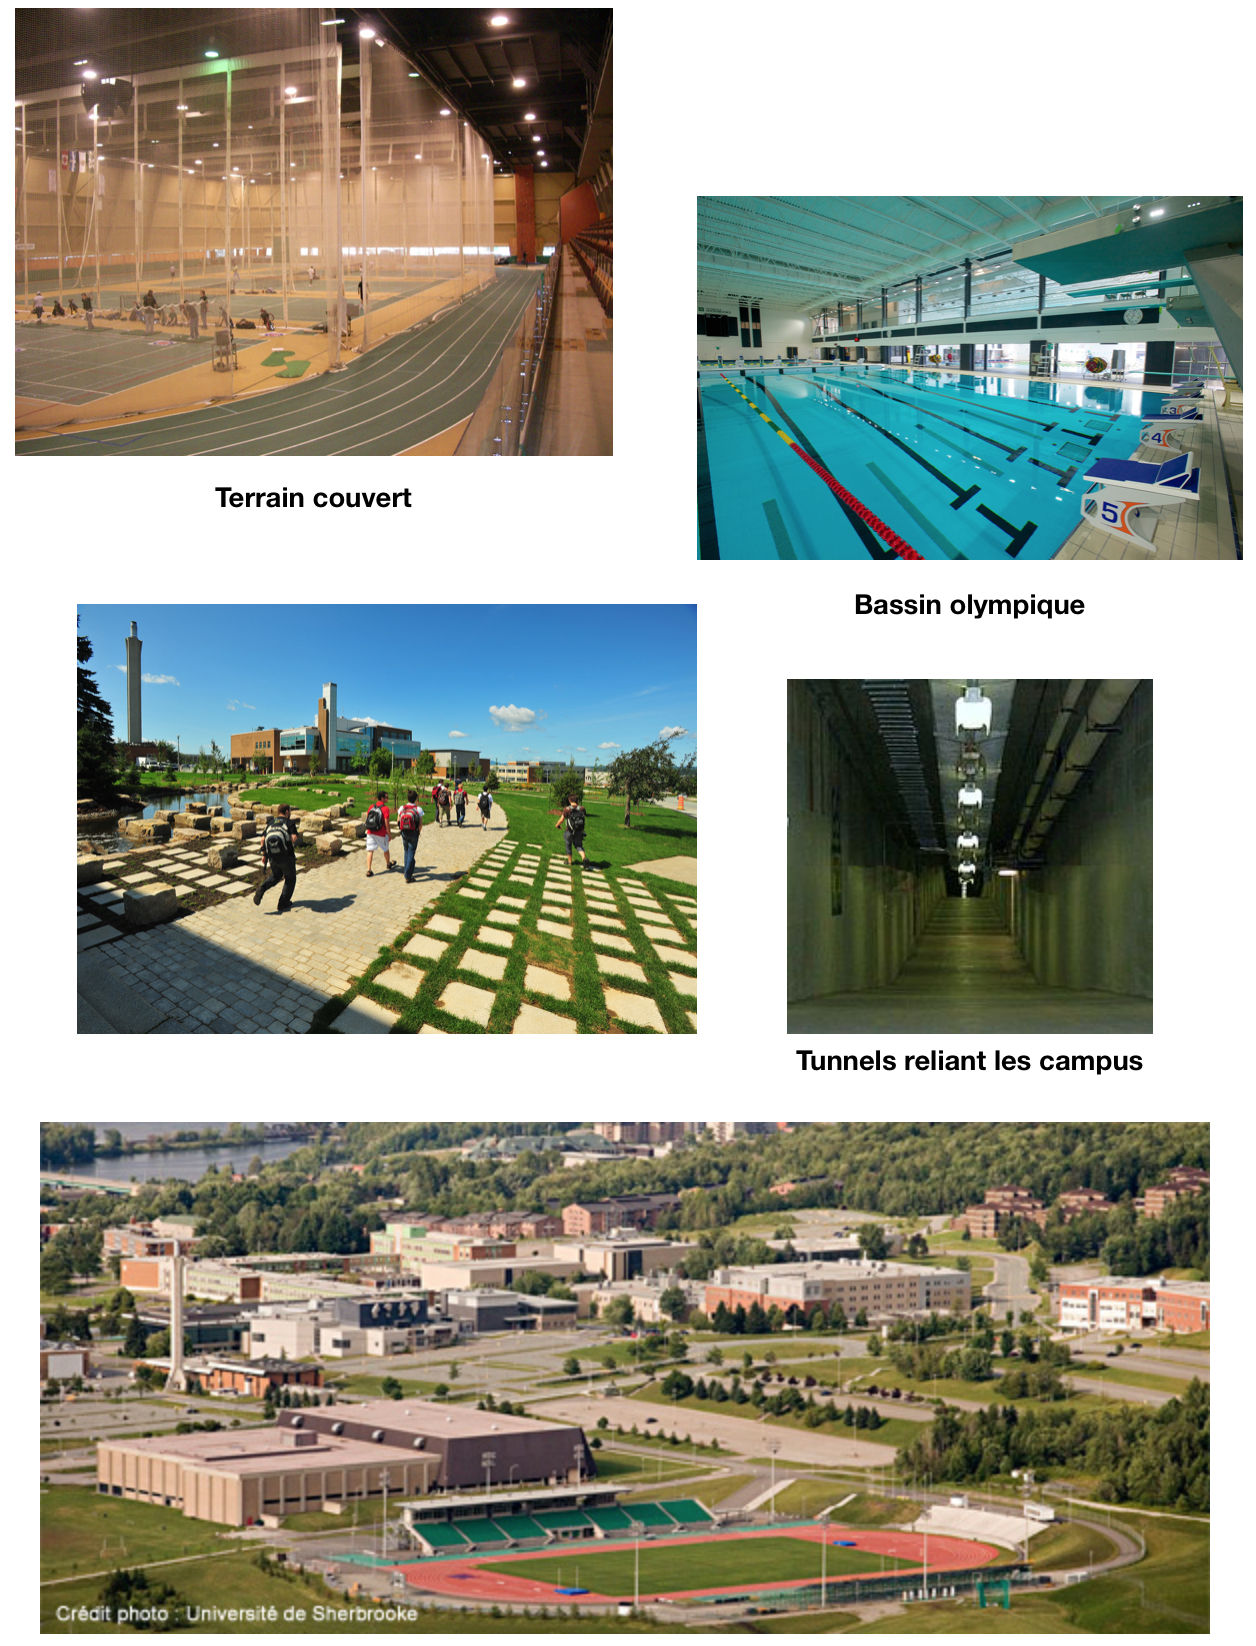
\includegraphics[width = 150mm]{figures/Image_Campus}
\caption{Très court aperçu du campus}
\end{figure}



\subsection{Les cours à l’université}\label{sec:sec4.7.1}

Au niveau des cours le fonctionnement est tout de même très différent de l'ESEO et il faut s'y habituer très rapidement. En général, vous aurez une quinzaine d'heures de cours par semaine ce qui sympas mais attention. Ici ils fonctionnent par lectures, c'est-à-dire que le prof vous donnera beaucoup d'information en très peu de temps dans ses cours, et vous donnera ensuite un guide de lecture pour la semaine. Un guide de lecture c'est une orientation que donne le professeur dans la lecture et la compréhension d'articles scientifiques publiés ou de livres. Cela n'a donc rien à voir avec ce que nous donne l'ESEO qui sont des pdf datant de l'avant-guerre ou des liens mort datant du minitel. Ceci est très intéressant car on apprend à rechercher l'information et avec divers supports et d'auteurs différents. On a donc plusieurs points de vue ce qui est très enrichissant. On a en moyenne une bonne centaine de pages à lire par semaine mais surtout à comprendre. Ce qui prend un temps considérable sur la semaine. Comptez 10 heures au moins la dessus. \\
Autre chose très importante, là bas tout se fait par la pratique. D'accord on lit beaucoup en dehors des cours, mais pendant c'est du Matlab, des calculs et de la pratique! \\
Pareil pour les examens. On se fait évaluer sur nos compétences sur Matlab même et pas sur un petit QCM ressemblant aux annales.\\
Je vous laisserai découvrir le reste par vous même.\\
À noter qu'ici il n'y a pas de rattrapage. C'est-à-dire que si vous louper une session, vous la repassez l'année prochaine ou à la prochaine session si elle est disponible. \\
Le système de notation est aussi différent ici, 10/20 ce n'est pas la moyenne ici, je vous laisse regarder le tableau suivant pour vous informer.


\begin{figure}[h!]
\centering
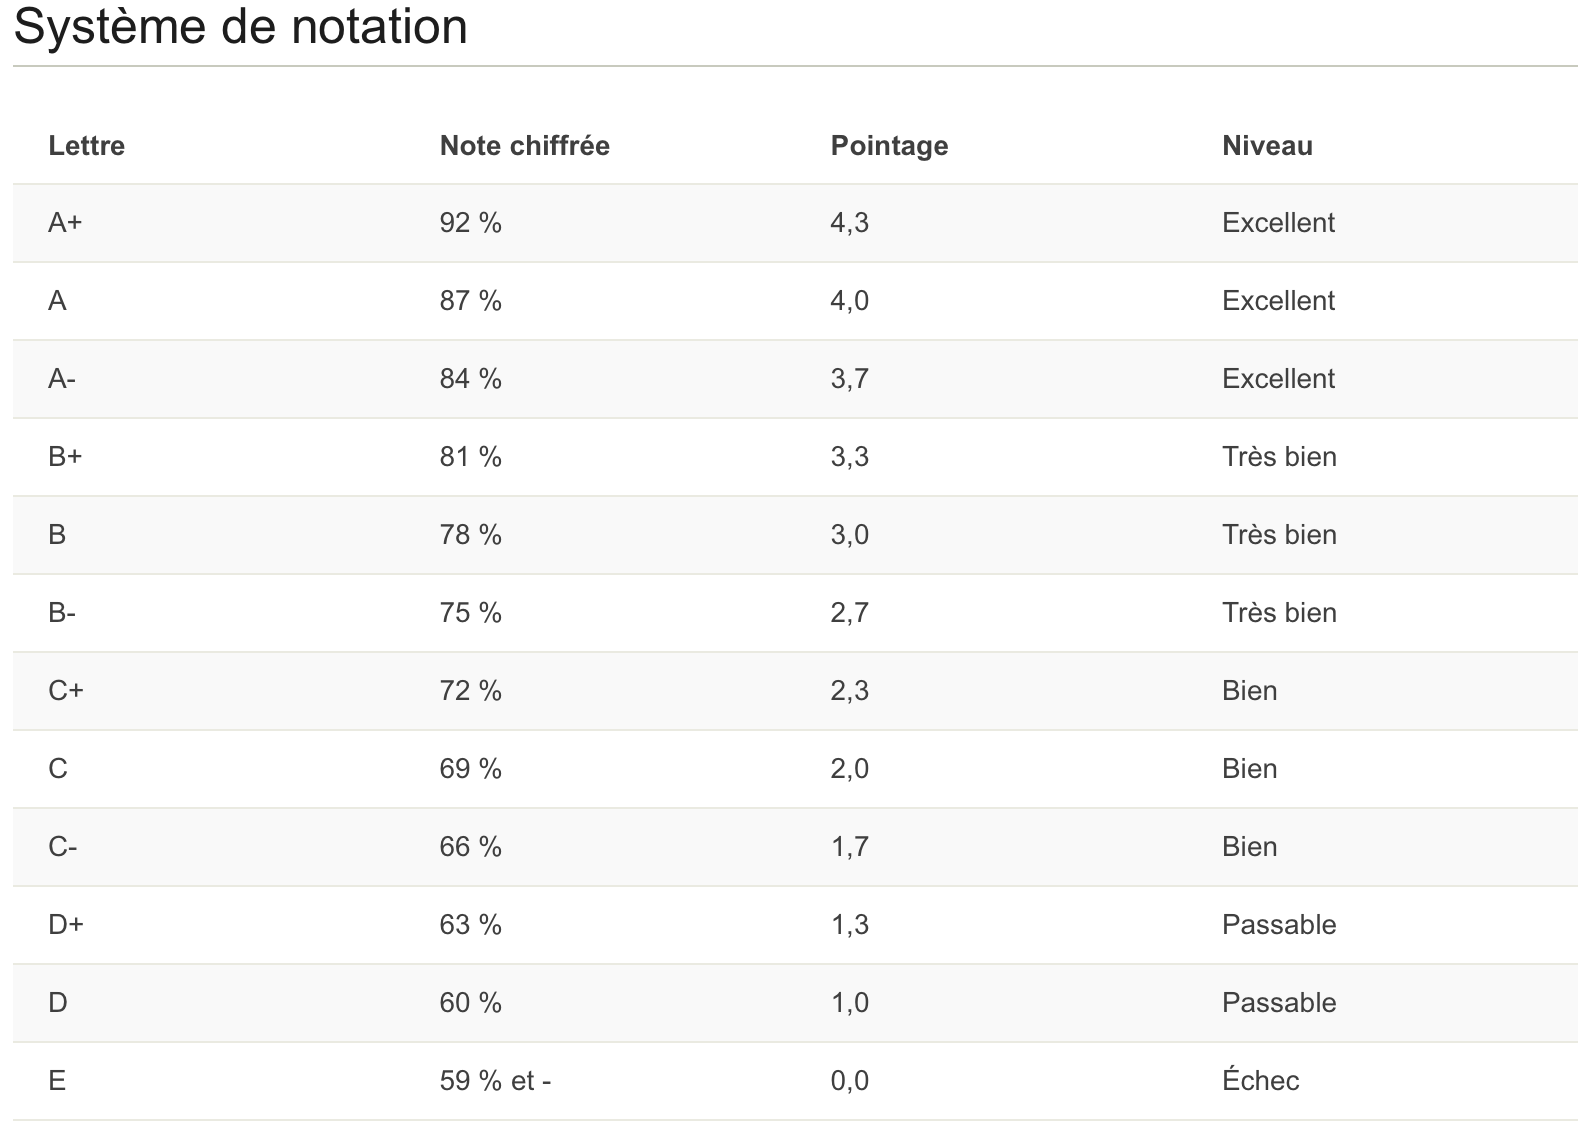
\includegraphics[width = 80mm]{figures/Sys_Notation}
\caption{Système de notation}
\end{figure}


\subsection{Un bidiplôme c’est bien, mais je veux plus!}\label{sec:sec4.7.2}

Vous avez pas prévu de revenir tout de suite? Pas de problème, les ingénieurs sont les bienvenues pour rester ici.

\subsubsection{Un doctorat}\label{sec:sec4.7.2.1}
Pour le doctorat, bien que non mentionné par l’ESEO, il est tout à fait envisageable ici. Le problème est que l’ESEO nous inscrit dans une maîtrise de type cours, et il faut être dans une maîtrise de type recherche pour y accéder.
Pas de panique, la passerelle existe entre ces deux sections à condition de trouver le professeur qui te prenne sous ton aile.
Il est possible de prévoir cela avant ton départ en prenant contact avec des professeurs d’ici, et en précisant bien que vous voulez une maîtrise de type cours à l’ESEO. Alors là je dis attention parce qu’avec les incompétents que vous avez en face de vous, la réponse varie du simple au double. Comme je l’ai dit avant, vous êtes seul alors surveillez bien vos arrières...

Si vous n’avez pas prévu cela avant de partir et que vous vous rendez, compte que ça serait quand même quelque chose qui vous intéresse, parlez-en à votre professeur référent lors de votre meeting pour votre choix de cours, il vous orientera sur les cours à prendre. Ensuite c’est à vous de trouver le domaine, et le professeur référent pour la thèse.

\begin{example}{Mon cas personnel}
  Je vais vous présenter mon cas, je suis inscrit en maîtrise de type cours et le doctorat était quelque chose qui m’intéressait, mais que je n’envisageais pas sérieusement. Or, après avoir vu les opportunités ici, cela m’a beaucoup fait réfléchir.
  Déjà, pourquoi un doctorat?
  \begin{itemize}
    \item Tout d’abord c’est le seul diplôme reconnu dans le monde entier. Ce qui est très intéressant si vous voulez voyager et pas rester dans le même bled paumé ou la même ville toute votre vie.
    \item Ensuite, votre thèse va être incroyablement formatrice dans l’approche et la résolution de problème très complexe. Un peu comme la prépa à grande petite échelle.
    \item Après, cela vous donne avant même d’être sorti une certaine connaissance et « renommée » dans le milieu scientifique, car vous commencez d’ores et déjà à publier des articles scientifiques.
    \item Un doctorat ne veut cependant pas dire professeur toute sa vie! Je l’entends beaucoup trop souvent et c’est faux, il y a une multitude de docteurs en entreprise et aussi un bon nombre de non-docteurs professeur! Regardez à l’ESEO vous allez être servie...
    \item Contrairement en France, le statut de doctorant est très bien vu partout dans le monde. Leur valeur est bien connue et cela se voit dans le salaire aussi. (Ça reste tout de même important même si nous ne sommes pas dans les sciences pour l’argent.)
    \item Une chose importante à mentionner cependant, je n’aurai pas accepté un doctorat à l’ESEO cependant. Tout simplement parce que le financement et les professeurs dernières sont complètement largués face aux autres pays. Ici tout va très vite, le budget est présent, pas besoin de 4 mois d’attente et de bataille avant d’avoir un générateur (j’image...). Les professeurs sont des références qui travaillent directement avec des entreprises comme Bombardier. C’est un très très gros plus.
  \end{itemize}

  J’ai donc fais part de cette envie avec Mr F.Maillot qui est mon professeur référent ici à Sherbrooke et il m’a orienté vers deux professeurs susceptibles de m’accueillir.
  Deux semaines plus tard après ma demande par e-mail, un des professeurs se manifeste et après une longue discussion concernant ma demande, mon parcours, le choix de mes cours, etc. Il serait en mesure de me proposer un doctorat pour l’année prochaine, à condition que je réussisse mon année à Sherbrooke sans accrocs. Le sujet de thèse remplit parfaitement mes envies et est particulièrement intéressant, tout cela s’accompagnant d’une bourse.
  Alors rien n’est fait, il y a des chances pour que je relise ce document dans deux ans et que je ne sois pas du tout en thèse à Sherbrooke, mais je veux juste vous partager mon expérience pour vous dire que c’est possible!
\end{example}

\subsubsection{Un travail}\label{sec:sec4.7.2.2}
La dernière nouvelle de l’ESEO est qu’il faut dorénavant effectuer un stage de 5 ou 6 mois (je ne me souviens plus bien) pour valider votre bidiplôme ici. Oui oui, on nous l’a dit un mois avant de partir...
Alors mise à part le fait qu’on nous prévient à la dernière minute, on peut tout de même en tirer du bon, surtout si vous voulez travailler ici.
À savoir que la recherche de stage ici se passe différemment qu’en France. Ici c’est l’entreprise qui vient te chercher. Je m’explique, chaque année les étudiants en recherche de stage remplissent une fiche avec l’annuaire des entreprises partenaires avec l’université. On oublie l’annuaire des entreprises qu’un certain « directeur des relations extérieures » garde précisément pour caler son bureau, ici on parle de vraies entreprises. L’étudiant choisit donc entre 28 entreprises (c’est ce que l’étudiant en question m’a dit donc à prendre avec des pincettes, car je ne peux pas vérifier avec plusieurs sources pour confirmer) et notre stage est trouvé parmi ces 28. En revanche je ne sais pas si cette méthode est disponible pour les étudiants étrangers, mais il n’y a pas de raison pour que cela ne se fasse pas. Si vous voulez continuer à travailler ici, c’est donc largement possible!
